\documentclass{standalone}
\usepackage{tikz}
\usetikzlibrary{shapes.geometric, arrows}

\definecolor{mycolor}{RGB}{0, 153, 255}
\tikzstyle{process} = [rectangle, rounded corners,
                       minimum width=2cm, minimum height=1cm,
                       text centered, draw=black, fill=mycolor,
                       text=white, line width=0.3mm]


\begin{document}
    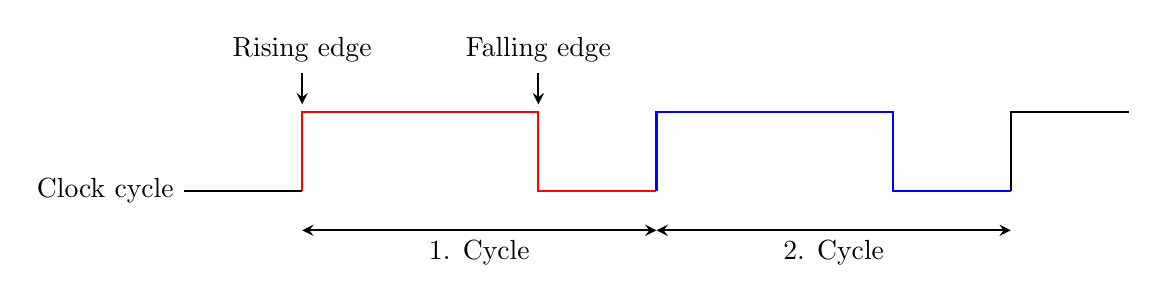
\begin{tikzpicture}[node distance=2cm]
        
        % Clock cycle graph
        \node at (-1,0) [text centered] (7) {Clock cycle};
        \draw [thick, color=black]  (0,0) -- ++(1.5,0);
        \draw [thick, color=red] (1.5, 0) -- ++(0,1) -- ++(3,0) -- ++(0,-1) -- ++(1.5,0);
        
        
        \draw [thick, color=blue] (6,0) -- ++(0,1) -- ++(3,0) -- ++(0,-1) -- ++(1.5,0);
        
        \draw [thick, color=black] (10.5,0) -- ++(0,1) -- ++(1.5,0) ;
        
        % First and second cycle arrows
        \draw [thick, <->,>=stealth] (1.5,-0.5) -- node [below] {1. Cycle} ++(4.5,0) ;
        \draw [thick, <->,>=stealth] (6,-0.5) -- node [below] {2. Cycle} ++(4.5,0) ;
        
        % Edges
        \node at (1.5,1.8) [text centered] (7) {Rising edge};
        \draw [thick, ->,>=stealth] (1.5,1.5) --  ++(0,-0.4) ;
        
        \node at (4.5,1.8) [text centered] (7) {Falling edge};
        \draw [thick, ->,>=stealth] (4.5,1.5) --  ++(0,-0.4) ;
        
%        %32 bit instruction
%        \node at (0,0) [text centered] (7) {0000};
%        \node at (1,0) [text centered] (6) {0000};
%        \node at (2,0) [text centered] (5) {1101};
%        \node at (3,0) [text centered] (4) {0110};
%        \node at (4,0) [text centered] (3) {0000};
%        \node at (5,0) [text centered] (2) {1001};
%        \node at (6,0) [text centered] (1) {0011};
%        \node at (7,0) [text centered] (0) {0011};
%        \node at (7.5,-0.1) [text centered] {$\; \texttt{\scriptsize two}$};
%        
        
        
%        %hex instrucion
%        \node at (1.75,-1.25) [text centered] (h) {0};
%        \node at (2.25  ,-1.25) [text centered] (g) {0};
%        \node at (2.75,-1.25) [text centered] (f) {d};
%        \node at (3.25  ,-1.25) [text centered] (e) {6};
%        \node at (3.75,-1.25) [text centered] (d) {0};
%        \node at (4.25  ,-1.25) [text centered] (c) {d};
%        \node at (4.75,-1.25) [text centered] (b) {3};
%        \node at (5.25  ,-1.25) [text centered] (a) {3};
%        
%        %Arrows
%        \draw [thick,<->,>=stealth] (7) |- (h);
%        \draw [thick,<->,>=stealth] (6) -- ++(0,-0.7) -- ++(1.25,0) -- (g);
%        \draw [thick,<->,>=stealth] (5) -- ++(0,-0.5) -- ++(0.75,0) -- (f);
%        \draw [thick,<->,>=stealth] (4) -- ++(0,-0.5) -- ++(0.25,0) -- (e);
%        \draw [thick,<->,>=stealth] (3) -- ++(0,-0.5) -- ++(-0.25,0) -- (d);
%        \draw [thick,<->,>=stealth] (2) -- ++(0,-0.5) -- ++(-0.75,0) -- (c);
%        \draw [thick,<->,>=stealth] (1) -- ++(0,-0.7) -- ++(-1.25,0) -- (b);
%        \draw [thick,<->,>=stealth] (0) |- (a);
%        \node at (5.5,-1.40) [text centered] {$\; \texttt{\scriptsize hex}$};
    
    \end{tikzpicture}
\end{document}
